% main.tex (revised)
\documentclass[11pt]{article}

% ==========================================================
% GLOBAL PACKAGES + CONFIG (EB)
% ==========================================================
% ==========================================================
% macros/packages.tex
% Electric Barometer (EB) — Global Packages
%
% Intent:
% - Centralize shared package imports and common configuration.
% - Keep ordering consistent across documents.
% - This file includes hyperref LAST. Do not load additional packages after
%   inputting this file in your main.tex.
% ==========================================================

% ----------------------------------------------------------
% Core typography & encoding
% ----------------------------------------------------------
\usepackage[T1]{fontenc}
\usepackage[utf8]{inputenc}
\usepackage{lmodern}

% ----------------------------------------------------------
% Page layout
% ----------------------------------------------------------
\usepackage[margin=1in]{geometry}

% ----------------------------------------------------------
% Mathematics
% ----------------------------------------------------------
\usepackage{amsmath}
\usepackage{amsfonts}
\usepackage{amssymb}

% ----------------------------------------------------------
% Tables & figures
% ----------------------------------------------------------
\usepackage{graphicx}
\usepackage{booktabs}

% Common utilities used across notes/papers
\usepackage{xcolor}
\usepackage{enumitem}

% Table helpers (used in some notes)
\usepackage{adjustbox}
\usepackage{tabularx}

% ----------------------------------------------------------
% TikZ & PGFPlots (standardized across EB)
% ----------------------------------------------------------
\usepackage{tikz}
\usetikzlibrary{
  arrows.meta,
  positioning,
  shapes.geometric,
  fit,
  calc,
  backgrounds,
  intersections
}

\usepackage{pgfplots}
\pgfplotsset{compat=1.18}
\usepgfplotslibrary{
  groupplots,
  fillbetween
}

% ----------------------------------------------------------
% Formatting utilities (used in multiple notes/papers)
% ----------------------------------------------------------
\usepackage{framed}
\usepackage{setspace}

% ----------------------------------------------------------
% Citations
% ----------------------------------------------------------
\usepackage[authoryear,round]{natbib}

% ----------------------------------------------------------
% Microtypography
% ----------------------------------------------------------
\usepackage{microtype}

% ----------------------------------------------------------
% Hyperlinks (MUST be loaded last)
% ----------------------------------------------------------
\usepackage[hidelinks]{hyperref}


% ==========================================================
% CUSTOM MACROS (shared notation)
% ==========================================================
% ==========================================================
% EB-PAPERS: CANONICAL MACROS / COMMANDS
% Forecast Readiness Framework (FRF) / Electric Barometer
% ==========================================================
% Goals:
% - One meaning per symbol.
% - Shared across all papers/notes/briefs.
% - Backwards-compatible aliases.
% - Avoid redefinition errors via \providecommand.
% ==========================================================

% ----------------------------------------------------------
% Core framework / artifacts
% ----------------------------------------------------------
\providecommand{\FRF}{\ensuremath{\mathrm{FRF}}}
\providecommand{\FRS}{\ensuremath{\mathrm{FRS}}}

\providecommand{\FPC}{\ensuremath{\mathrm{FPC}}}
\providecommand{\DQC}{\ensuremath{\mathrm{DQC}}}
\providecommand{\Governance}{\ensuremath{\mathrm{Governance}}}
\providecommand{\GovernanceDecision}{\ensuremath{\mathrm{GovernanceDecision}}}

\providecommand{\RAL}{\ensuremath{\mathrm{RAL}}}

% Readiness primitives / governance vocabulary
\providecommand{\ReadinessPrimitive}{\ensuremath{\mathrm{RP}}}

% Limited-Time Offers
\providecommand{\LTO}{\ensuremath{\mathrm{LTO}}}
\providecommand{\LTOs}{\ensuremath{\mathrm{LTOs}}}

% ----------------------------------------------------------
% Core metrics (upright math)
% ----------------------------------------------------------
\providecommand{\CWSL}{\ensuremath{\mathrm{CWSL}}}
\providecommand{\CWSLR}{\ensuremath{\mathrm{CWSLR}}} % named artifact in prose
\providecommand{\NSL}{\ensuremath{\mathrm{NSL}}}
\providecommand{\UD}{\ensuremath{\mathrm{UD}}}
\providecommand{\HR}{\ensuremath{\mathrm{HR}}}
\providecommand{\HRtau}{\ensuremath{\mathrm{HR}@\tau}}

% FRS sub-terms
\providecommand{\CWSLscaled}{\ensuremath{\mathrm{CWSL}_{\mathrm{scaled}}}}
\providecommand{\CWSLmax}{\ensuremath{\mathrm{CWSL}_{\max}}}

% Legacy HR macro names
\providecommand{\HRAT}{\ensuremath{\mathrm{HR@\tau}}}
\providecommand{\tauTol}{\ensuremath{\tau}}
\providecommand{\tauop}{\ensuremath{\tau}}

% ----------------------------------------------------------
% Indexing and sets
% ----------------------------------------------------------
\providecommand{\Iset}{\ensuremath{I}}
\providecommand{\Tset}{\ensuremath{T}}

\providecommand{\entity}{\ensuremath{i}}
\providecommand{\timeindex}{\ensuremath{t}}

% Back-compat index shorthands
\providecommand{\iidx}{\entity}
\providecommand{\tidx}{\timeindex}

% Summation shorthand
\providecommand{\sumit}{\ensuremath{\sum_{\entity \in \Iset} \sum_{\timeindex \in \Tset}}}

% Optional sizes / counts
\providecommand{\Tsize}{\ensuremath{|\Tset|}}
\providecommand{\nobs}{\ensuremath{N}}

% ----------------------------------------------------------
% Forecast / demand notation
% ----------------------------------------------------------
\providecommand{\y}{\ensuremath{y}}
\providecommand{\yhat}{\ensuremath{\hat{y}}}

\providecommand{\yit}{\ensuremath{y_{\entity\timeindex}}}
\providecommand{\yhatit}{\ensuremath{\hat{y}_{\entity\timeindex}}}

% Common residuals / errors
\providecommand{\errit}{\ensuremath{e_{\entity\timeindex}}}
\providecommand{\resit}{\errit} % alias
\providecommand{\absit}{\ensuremath{\left|\yhatit - \yit\right|}}
\providecommand{\abserrit}{\absit} % alias

% Explicit residual definition macro (optional)
\providecommand{\resdef}{\ensuremath{\errit = \yit - \yhatit}}

% ----------------------------------------------------------
% Shortfall / overbuild decomposition
% ----------------------------------------------------------
\providecommand{\shortfall}{\ensuremath{s}}
\providecommand{\overbuild}{\ensuremath{o}}

\providecommand{\sit}{\ensuremath{s_{\entity\timeindex}}}
\providecommand{\oit}{\ensuremath{o_{\entity\timeindex}}}

% Positive-part operator (canonical name)
\providecommand{\pospart}[1]{\left(#1\right)_{+}}

% Explicit decompositions
\providecommand{\shortfalldef}{\ensuremath{\sit = \pospart{\yit - \yhatit}}}
\providecommand{\overbuilddef}{\ensuremath{\oit = \pospart{\yhatit - \yit}}}

% Back-compat convenience symbols used in some notes
\providecommand{\sdepth}{\shortfall} % UD paper convenience

% ----------------------------------------------------------
% Indicators / expectations / operators
% ----------------------------------------------------------
% Canonical indicator: \Ind{event}
\providecommand{\Ind}{\ensuremath{\mathbb{I}}}
\providecommand{\indicator}[1]{\ensuremath{\mathbf{1}\{#1\}}} % prose-friendly alternative

% Back-compat: some notes used \Indicator (capital I). Keep as an alias to the
% canonical \Ind to avoid duplicate meanings.
\providecommand{\Indicator}{\Ind}

% If you want function-style indicator without braces: \Ind\!(event)
% Keep as \Ind and let authors decide.
\providecommand{\E}{\ensuremath{\mathbb{E}}}

\providecommand{\abs}[1]{\left|#1\right|}
\providecommand{\card}[1]{\left|#1\right|}

% ----------------------------------------------------------
% Cost parameters + cost ratio calibration (CWSLR note)
% ----------------------------------------------------------
% IMPORTANT: Canonical costs are subscripted (c_u, c_o). This avoids
% collisions with superscript variants.
\providecommand{\cu}{\ensuremath{c_u}}
\providecommand{\co}{\ensuremath{c_o}}

% Entity-specific costs
\providecommand{\cui}{\ensuremath{c_{u,\entity}}}
\providecommand{\coi}{\ensuremath{c_{o,\entity}}}

% Cost ratio
\providecommand{\R}{\ensuremath{R}}
\providecommand{\Ri}{\ensuremath{R_{\entity}}}
\providecommand{\Rdef}{\ensuremath{R = \cu/\co}}

% Aggregate under/over cost functions (used in calibration prose)
\providecommand{\UnderCost}{\ensuremath{\mathrm{UnderCost}}}
\providecommand{\OverCost}{\ensuremath{\mathrm{OverCost}}}

% Candidate grid
\providecommand{\Rgrid}{\ensuremath{\mathcal{R}}}

% Calibrated selections
\providecommand{\Rstar}{\ensuremath{R^{\ast}}}
\providecommand{\Rist}{\ensuremath{R^{\ast}_{\entity}}}

% CWSL as a function of R (notation)
\providecommand{\CWSLofR}{\ensuremath{\CWSL(\R)}}
\providecommand{\CWSLofRi}{\ensuremath{\CWSL(\Ri)}}

% Balance-based selection operator (kept as a macro because you used it)
\providecommand{\Rbalance}{%
\ensuremath{%
\arg\min_{\R \in \Rgrid}\left|\UnderCost(\R) - \OverCost(\R)\right|%
}%
}

% Back-compat (older notes used superscripts c^u / c^o)
\providecommand{\cuSup}{\ensuremath{c^{u}}}
\providecommand{\coSup}{\ensuremath{c^{o}}}
\providecommand{\cuiSup}{\ensuremath{c^{u}_{\entity}}}
\providecommand{\coiSup}{\ensuremath{c^{o}_{\entity}}}

% ----------------------------------------------------------
% HR@tau scanning / calibration (HRtau note)
% ----------------------------------------------------------
\providecommand{\tauval}{\ensuremath{\tau}}
\providecommand{\tauv}{\tauval}
\providecommand{\taui}{\ensuremath{\tau_{\entity}}}

% Candidate tolerance grid
\providecommand{\TauGrid}{\ensuremath{\mathcal{T}}}

% Calibrated tolerances
\providecommand{\taustar}{\ensuremath{\tau^{\ast}}}
\providecommand{\taustari}{\ensuremath{\tau^{\ast}_{\entity}}}

% Target hit-rate (if used)
\providecommand{\hstar}{\ensuremath{h^{\ast}}}

% Hit indicator definition helpers
\providecommand{\Hitit}{\ensuremath{h_{\entity\timeindex}}}
\providecommand{\HitDef}{\ensuremath{\Hitit = \Ind\!\left(\absit \le \tauval\right)}}

% HR as a function of tau
\providecommand{\HRoftau}{\ensuremath{\HR(\tauval)}}
\providecommand{\HRtauoftau}{\ensuremath{\HRtau(\tauval)}}

% Optional utility selection helpers
\providecommand{\lambdau}{\ensuremath{\lambda}}
\providecommand{\taumax}{\ensuremath{\tau_{\max}}}
\providecommand{\Utility}{\ensuremath{\mathcal{U}}}
\providecommand{\UtilityDef}{\ensuremath{\Utility(\tauval) = \HR(\tauval) - \lambdau \cdot (\tauval/\taumax)}}

% Governance guards
\providecommand{\taufloor}{\ensuremath{\tau_{\min}}}
\providecommand{\taucap}{\ensuremath{\tau_{\mathrm{cap}}}}
\providecommand{\nmin}{\ensuremath{n_{\min}}}

% ----------------------------------------------------------
% DQC / snapping / quantization (DQC note)
% ----------------------------------------------------------
\providecommand{\gunit}{\ensuremath{g}}
\providecommand{\guniti}{\ensuremath{g_{\entity}}}

\providecommand{\ygrid}{\ensuremath{\tilde{y}}}
\providecommand{\ygridit}{\ensuremath{\tilde{y}_{\entity\timeindex}}}

\providecommand{\yhatgrid}{\ensuremath{\tilde{\hat{y}}}}
\providecommand{\yhatgridit}{\ensuremath{\tilde{\hat{y}}_{\entity\timeindex}}}

\providecommand{\snap}{\ensuremath{\mathcal{S}}}
\providecommand{\snaphatdef}{\ensuremath{\yhatgridit = \snap_{\gunit}\!\left(\yhatit\right)}}
\providecommand{\snapydef}{\ensuremath{\ygridit = \snap_{\gunit}\!\left(\yit\right)}}

\providecommand{\residit}{\ensuremath{r_{\entity\timeindex}}}
\providecommand{\residdef}{\ensuremath{\residit = \yit - \ygridit}}

\providecommand{\MAD}{\ensuremath{\mathrm{MAD}}}
\providecommand{\IQR}{\ensuremath{\mathrm{IQR}}}

\providecommand{\multirate}{\ensuremath{\rho}}
\providecommand{\multiratei}{\ensuremath{\rho_{\entity}}}

\providecommand{\DeltaStar}{\ensuremath{\Delta^{\ast}}}

\providecommand{\Pset}{\ensuremath{\mathcal{P}}}
\providecommand{\packunit}{\ensuremath{p}}
\providecommand{\packuniti}{\ensuremath{p_{\entity}}}

% DQC classes
\providecommand{\ContinuousLike}{\textsc{Continuous-like}}
\providecommand{\Quantized}{\textsc{Quantized}}
\providecommand{\PiecewisePacked}{\textsc{Piecewise-packed}}

% FPC classes
\providecommand{\Compatible}{\textsc{Compatible}}
\providecommand{\Marginal}{\textsc{Marginal}}
\providecommand{\Incompatible}{\textsc{Incompatible}}

% ----------------------------------------------------------
% RAL shorthands used in notes
% ----------------------------------------------------------
\providecommand{\alphaadj}{\ensuremath{\alpha}}

% RAL operator (functional form)
\providecommand{\RALop}{\ensuremath{\mathcal{R}_{\alphaadj}}}

\providecommand{\yhatadjit}{\ensuremath{\hat{y}^{(\alphaadj)}_{\entity\timeindex}}}
\providecommand{\yhatadjdef}{\ensuremath{\yhatadjit = (1+\alphaadj)\,\yhatit}}

\providecommand{\dNSL}{\ensuremath{\Delta \NSL}}
\providecommand{\dHRtau}{\ensuremath{\Delta \HRtau}}
\providecommand{\dCWSL}{\ensuremath{\Delta \CWSL}}

% ----------------------------------------------------------
% Governance policy handles
% ----------------------------------------------------------
\providecommand{\TauPolicy}{\ensuremath{\mathrm{TauPolicy}}}
\providecommand{\RALPolicy}{\ensuremath{\mathrm{RALPolicy}}}
\providecommand{\UnitPolicy}{\ensuremath{\mathrm{UnitPolicy}}}

\providecommand{\GovernanceStatus}{\ensuremath{\mathrm{GovernanceStatus}}}
\providecommand{\Green}{\textsc{Green}}
\providecommand{\Yellow}{\textsc{Yellow}}
\providecommand{\Red}{\textsc{Red}}

\providecommand{\RawUnits}{\textsc{Raw}}
\providecommand{\SnappedUnits}{\textsc{Snapped}}

% ----------------------------------------------------------
% LTO paper specifics
% ----------------------------------------------------------
\providecommand{\ltoOn}{\ensuremath{z_{\timeindex}}}
\providecommand{\ltoPhase}{\ensuremath{\phi_{\timeindex}}}
\providecommand{\qprod}{\ensuremath{\mathrm{QP}}}

% ----------------------------------------------------------
% Frontmatter helpers
% ----------------------------------------------------------
\providecommand{\keywords}[1]{%
\par\noindent\textbf{Keywords: }#1\par
}

% ----------------------------------------------------------
% Prose shorthands
% ----------------------------------------------------------
\providecommand{\ie}{i.e.\ }
\providecommand{\eg}{e.g.\ }

% ==========================================================
% END
% ==========================================================


% ==========================================================
% STYLE LAYER (EB)
% ==========================================================
% ==========================================================
% macros/style.tex
% Electric Barometer — Style Layer (v1)
% ----------------------------------------------------------
% Scope (v1):
%   - PDF metadata only
%
% Notes:
%   - Assumes hyperref is already loaded via macros/packages.tex
%   - This file should NOT load packages.
% ==========================================================

% ----------------------------------------------------------
% PDF METADATA (canonical helper)
% ----------------------------------------------------------
% Usage:
%   \EBPdfMeta{<pdftitle>}{<pdfauthor>}{<pdfsubject>}{<pdfkeywords>}
%
% Examples:
%   \EBPdfMeta
%     {Cost-Weighted Service Loss (CWSL): An Asymmetric Cost Metric for Forecast Evaluation}
%     {Kyle Corrie}
%     {Technical Note — Electric Barometer Series}
%     {Electric Barometer, Forecast Readiness Framework, CWSL, asymmetric loss}
%
\newcommand{\EBPdfMeta}[4]{%
  \hypersetup{%
    pdftitle={#1},%
    pdfauthor={#2},%
    pdfsubject={#3},%
    pdfkeywords={#4},%
    colorlinks=true,%
    linkcolor=blue,%
    citecolor=blue,%
    urlcolor=blue%
  }%
}


% ==========================================================
% PDF METADATA
% ==========================================================
\EBPdfMeta
  {Cost Ratio Sensitivity and Calibration for Cost-Weighted Service Loss}
  {Kyle Corrie}
  {Technical Note --- Electric Barometer Series}
  {Electric Barometer, Forecast Readiness Framework, CWSL, cost ratio, calibration, sensitivity analysis, asymmetric loss}

% ==========================================================
% TITLE BLOCK
% ==========================================================
\title{
\textbf{Cost Ratio Sensitivity and Calibration for \CWSL}\\[4pt]
{\large Governing Cost Asymmetry in Forecast Evaluation}
}

\author{
  Kyle Corrie\\[4pt]
  \small Forecast Readiness Framework (FRF)\\
  \small Electric Barometer Series
}

\date{January 2026\\[4pt]
\small Technical Note --- Electric Barometer Series\\
Version 1.1}

% ==========================================================
\begin{document}

\maketitle

% ==========================================================
% FRONTMATTER
% ==========================================================
% ==========================================================
% 000_frontmatter.tex
% FRONTMATTER (Forecast Governance Technical Note)
% ==========================================================

\begin{abstract}
Operational forecasting systems increasingly embed evaluation diagnostics directly
into downstream decisions, policy gates, and automated readiness interventions.
In such settings, it is not sufficient to compute cost-aware error or service
metrics. One must also establish that both the \emph{units of interpretation} and
the \emph{forecast primitive itself} are structurally admissible for the observed
demand process.

This technical note introduces \emph{Forecast Governance} as a deterministic,
auditable decision contract that composes two companion diagnostics:
\emph{Demand Quantization Compatibility (DQC)}, which determines whether evaluation
and control must respect a discrete demand representation, and
\emph{Forecast Primitive Compatibility (FPC)}, which determines whether readiness
adjustment constitutes a valid control lever under that representation.

Governance produces a single authoritative artifact—the
\texttt{GovernanceDecision}—that specifies representation requirements, tolerance
semantics, readiness allowability, and compliance status with explicit rationale.
Forecast Governance is not a performance metric and is not an optimization
objective. It is a policy layer designed to ensure that evaluation semantics are
well-defined before downstream optimization, selection, or control is attempted.
\end{abstract}


% ==========================================================
% ORDERED SECTION INPUTS (Technical Note Schema)
% ==========================================================
% ==========================================================
% 010_overview.tex
% Overview
% ==========================================================

\section{Overview}
\label{sec:governance_overview}

Modern operational forecasting systems increasingly embed automated control
levers, tolerance-based evaluation, and asymmetric cost tradeoffs directly into
decision workflows. In such settings, analytic diagnostics alone are
insufficient. What ultimately matters is not whether a forecast appears
reasonable, but whether a downstream action is \emph{structurally admissible},
\emph{policy-compliant}, and \emph{accountable}.

Within the Electric Barometer framework, this responsibility is assigned to
\emph{Governance}. Governance is the final decision layer that binds structural
diagnostics into an authoritative operational outcome. It does not generate new
signals, optimize objectives, or reinterpret performance. Instead, it resolves
diagnostic inputs into a single, enforceable policy decision.

This technical note formalizes governance as a deterministic \emph{decision
contract}. Given a fixed set of diagnostic inputs and thresholds, governance
produces exactly one authoritative artifact that specifies:
\begin{itemize}[leftmargin=1.5em]
  \item the admissible unit system for interpretation,
  \item the authoritative tolerance semantics,
  \item the allowability of readiness adjustment,
  \item and an explicit governance status.
\end{itemize}

Governance consumes—but does not redefine—two upstream diagnostics:
\begin{itemize}[leftmargin=1.5em]
  \item \textbf{Demand Quantization Compatibility (DQC)}, which determines whether
        realized demand admits continuous interpretation or requires discrete,
        grid-aware semantics; and
  \item \textbf{Forecast Primitive Compatibility (FPC)}, which determines whether
        a forecast primitive can respond coherently to readiness adjustment under
        admissible perturbations.
\end{itemize}

Crucially, governance does not average, negotiate, or arbitrate between these
diagnostics. It enforces strict exclusivity: one unit system governs, one
diagnostic interpretation is authoritative, and one readiness policy applies.
When required inputs are missing or incompatible, governance fails explicitly
rather than degrading silently.

The purpose of this design is closure. Governance exists to \emph{terminate
interpretation, not extend it}: once a \texttt{GovernanceDecision} is issued, no
further diagnostic reasoning is admissible.

By enforcing this closure, governance prevents common operational failure modes
such as:
\begin{itemize}[leftmargin=1.5em]
  \item mixing raw and snapped evaluation semantics,
  \item interpreting tolerances smaller than realizable demand increments,
  \item applying readiness adjustments that cannot be operationally executed.
\end{itemize}

This note describes the governance contract, the structure of the decision
artifact it emits, the deterministic logic by which decisions are made, and the
interpretive boundaries that preserve accountability. Together with the DQC and
FPC technical notes, it completes the Electric Barometer framework by ensuring
that readiness decisions are not only cost-aware or service-aware, but
\emph{structurally valid, auditable, and enforceable by design}.

% ----------------------------------------------------------
% OPERATIONAL PROBLEM
% ----------------------------------------------------------
\section{Tolerance as an Operational Decision}
\label{sec:operational_problem}

Tolerance-based metrics such as \HRtau{} evaluate forecast performance by
counting the fraction of observations whose absolute error falls within an
acceptable band.
While simple to compute and easy to interpret, the practical meaning of
\HRtau{} depends entirely on the choice of the tolerance parameter $\tauv$.
Despite this dependence, $\tauv$ is often selected informally or treated as an
arbitrary constant.

In many operational settings, tolerance thresholds are chosen based on
convention (e.g., ``within one unit'' or ``within 10\%''), borrowed from prior
analyses, or tuned implicitly to produce desired hit rates.
Such practices obscure the role of tolerance as a policy decision rather than a
statistical artifact.
Once forecasts are used to drive production, staffing, or service commitments,
the choice of $\tauv$ directly determines what constitutes acceptable
performance.

Crucially, $\tauv$ is not a modeling hyperparameter in the usual sense.
It does not affect how forecasts are generated, nor does it alter their
statistical fit to observed data.
Instead, $\tauv$ encodes an \emph{operational acceptability standard}: the maximum
deviation from realized demand that can be tolerated without triggering
material consequences.
As such, specifying $\tauv$ is a governance decision that shapes readiness
assessment and downstream decision-making.
This perspective aligns with established work on forecast evaluation, which
emphasizes that performance metrics must be interpreted relative to the loss or
decision structure induced by their downstream use \citep{gneiting2011}.

\subsection{Consequences of mis-specifying tolerance}
\label{subsec:mis_specification}

Mis-specification of $\tauv$ can materially distort evaluation outcomes.
When $\tauv$ is set too narrowly, small and operationally insignificant errors
are counted as failures, exaggerating forecast volatility and penalizing
otherwise adequate models.
When $\tauv$ is set too broadly, large errors are absorbed into the tolerance
band, masking readiness risks and creating a false sense of stability.

Because \HRtau{} aggregates binary hit events, these effects are nonlinear.
Small changes in $\tauv$ can produce abrupt changes in hit rate, particularly
when error distributions are concentrated near the tolerance boundary.
As a result, model rankings and readiness conclusions may depend more on the
chosen tolerance than on intrinsic forecast quality.

\subsection{Why optimization is the wrong framing}
\label{subsec:why_not_optimization}

It may be tempting to select $\tauv$ by optimizing \HRtau{} directly, choosing
the tolerance that achieves a target hit rate or maximizes apparent coverage.
This framing is misleading.
Increasing $\tauv$ monotonically increases hit rate, making unconstrained
optimization trivial and operationally meaningless.

Even when forecasting models themselves are trained with asymmetric or
quantile-based loss functions, the evaluation tolerance $\tauv$ remains a
distinct governance choice.
It determines how forecast error is judged after predictions are produced, not
how predictions are learned.

The appropriate question is therefore not
``Which $\tauv$ maximizes \HRtau{}?''
but rather
``Which tolerance reflects a defensible boundary between acceptable and
unacceptable error given historical behavior?''

\subsection{Toward governed tolerance selection}
\label{subsec:governed_tolerance}

From an operational perspective, tolerance calibration should make acceptability
standards explicit, inspectable, and auditable.
A governed approach to tolerance selection should:
\begin{itemize}[leftmargin=*]
    \item expose how hit rates vary across plausible tolerance values,
    \item avoid tolerance inflation driven by noise or convenience,
    \item rely only on historical forecast errors,
    \item support consistent application across entities and time periods.
\end{itemize}

These requirements motivate a sensitivity- and calibration-based treatment of
$\tauv$, in which \HRtau{} is evaluated across a candidate tolerance grid and
selection rules are defined in terms of observable error structure rather than
numerical maximization.
The next sections formalize this perspective by framing \HRtau{} as a response
surface over tolerance and introducing governed calibration mechanisms.
% ----------------------------------------------------------
% CWSL RESPONSE SURFACE
% ----------------------------------------------------------
\section{\CWSL{} as a Function of Cost Asymmetry}
\label{sec:response_surface}

Although \CWSL{} is typically reported at a single cost ratio $\R$, the metric is
more naturally understood as a \emph{response surface} over cost asymmetry.
For fixed forecast outcomes $(y_{it}, \hat{y}_{it})$ and a fixed overbuild cost
$\co$, \CWSL{} can be written explicitly as a function of $\R$ by setting
$\cu = \R \cdot \co$:
\[
    \CWSLR = 
    \frac{
        \sumit
        \left[
            \R \cdot \co \cdot \sit
            +
            \co \cdot \oit
        \right]
    }{
        \sumit \yit
    }.
\]
This representation makes clear that \CWSL{} is not a single scalar quantity, but
a family of values indexed by $\R$.

\subsection{Structure of the response surface}
\label{subsec:surface_structure}

For any fixed dataset, \CWSLR{} is a deterministic, piecewise-linear function of
$\R$.
The overbuild component is independent of $\R$, while the underbuild component
scales linearly with $\R$.
As a result, the shape of the response surface is governed entirely by the
distribution and magnitude of historical shortfalls relative to overbuild.

Several qualitative regimes are common in practice:
\begin{itemize}[leftmargin=*]
    \item \textbf{Underbuild-dominated regimes}, where \CWSLR{} increases rapidly
    with $\R$, indicating that shortfalls are frequent or deep.
    \item \textbf{Overbuild-dominated regimes}, where \CWSLR{} is relatively flat
    for moderate $\R$, reflecting excess capacity or conservative forecasting.
    \item \textbf{Mixed regimes}, where curvature changes across the range of
    $\R$, suggesting a tradeoff between shortfall and surplus that depends on
    cost assumptions.
\end{itemize}

These regimes are properties of the historical forecast errors, not of the
forecasting model itself. Consequently, interpreting \CWSL{} at a single
$\R$ without inspecting the surrounding response surface can obscure important
operational behavior.

\subsection{Why response surfaces matter}
\label{subsec:why_surface}

Viewing \CWSL{} as a response surface clarifies two practical points.
First, robustness to cost assumptions can be assessed directly by examining how
rapidly \CWSLR{} changes across plausible values of $\R$.
Flat regions indicate stability: evaluation conclusions are unlikely to change
materially if the true operational cost ratio differs modestly from the assumed
one.
Steep regions indicate fragility: small changes in $\R$ can lead to large changes
in measured performance or model ranking.

Second, the response-surface view separates \emph{evaluation} from
\emph{calibration}.
Rather than selecting $\R$ to minimize \CWSL{}, we can ask how underbuild and
overbuild costs balance across $\R$, and where that balance yields an
operationally interpretable reference point.
This perspective motivates grid-based sensitivity analysis as a first-class
diagnostic, rather than an auxiliary experiment.

The next section formalizes this idea by introducing a grid-based procedure for
evaluating \CWSL{} across a candidate set of cost ratios and extracting
sensitivity diagnostics from the resulting response curve.
% ----------------------------------------------------------
% SENSITIVITY ANALYSIS
% ----------------------------------------------------------
\section{Grid-Based Sensitivity Analysis}
\label{sec:sensitivity_analysis}

To operationalize the response-surface view of \CWSL{}, we evaluate the metric
across a finite, user-specified grid of candidate cost ratios
$\Rgrid = \{\R_1, \R_2, \ldots, \R_K\}$.
Rather than committing to a single asymmetry assumption, this procedure exposes
how evaluation outcomes vary as $\R{}$ changes, enabling explicit robustness and
stability checks.

This perspective aligns with established principles of sensitivity analysis,
which emphasize understanding how conclusions depend on uncertain assumptions
rather than optimizing parameters in isolation \citep{saltelli2008}.

\subsection{Candidate grid construction}
\label{subsec:grid_construction}

The grid $\Rgrid$ should span the range of cost asymmetries considered plausible
for the application domain.
In practice, $\Rgrid$ is typically chosen as a small set of positive values,
for example $\{0.5, 1.0, 2.0, 3.0\}$ or a denser logarithmic sequence when finer
resolution is required.
The methods discussed here do not rely on any particular spacing or distribution
of grid points; determinism is ensured as long as the grid is fixed.

Importantly, sensitivity analysis does not require that the ``true'' cost ratio
lie exactly on the grid.
The purpose of $\Rgrid$ is not precise estimation, but controlled exploration of
how conclusions change across a range of assumptions.
For this reason, the candidate grid itself should be treated as a governed
artifact, recorded and reported alongside evaluation outputs to ensure
reproducibility and transparency in downstream decision-making.

\subsection{Evaluating the sensitivity curve}
\label{subsec:sensitivity_curve}

For each $\R_k \in \Rgrid$, we compute $\CWSL(\R_k)$ using identical data and
normalization.
The resulting set of pairs
\[
    \{(\R_k, \CWSL(\R_k))\}_{k=1}^{K}
\]
defines a discrete approximation to the continuous response surface discussed in
Section~\ref{sec:response_surface}.

% --- Figure: response surface over the governed grid ---
% ----------------------------------------------------------
% FIGURE: CWSL response surface vs cost ratio R
% ----------------------------------------------------------
\begin{figure}[t]
\centering
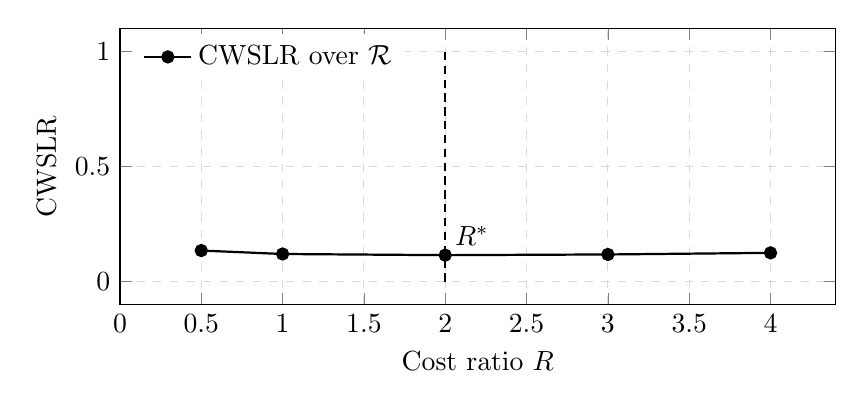
\begin{tikzpicture}
\begin{axis}[
    width=0.88\textwidth,
    height=0.42\textwidth,
    xlabel={Cost ratio $\R{}$},
    ylabel={$\CWSLR{}$},
    xmin=0,
    ymajorgrids=true,
    xmajorgrids=true,
    grid style={dashed,gray!30},
    legend style={draw=none, at={(0.02,0.98)}, anchor=north west},
    legend cell align={left},
]

% --- Placeholder curve (replace with your computed values) ---
% Example grid: R in {0.5, 1.0, 2.0, 3.0, 4.0}
\addplot[
    thick,
    mark=*,
]
coordinates {
    (0.5, 0.135)
    (1.0, 0.120)
    (2.0, 0.115)
    (3.0, 0.118)
    (4.0, 0.125)
};
\addlegendentry{$\CWSLR{}$ over $\Rgrid{}$}

% --- Optional: show calibrated R* as a vertical marker ---
% Replace 2.0 with your calibrated \Rstar{} value.
\addplot[densely dashed, thick] coordinates {(2.0, 0.0) (2.0, 1.0)};
\node[anchor=south west] at (axis cs:2.0, 0.115) {$\Rstar{}$};

% --- Optional: show a "business-chosen" R as a dotted marker ---
% Uncomment and replace 3.0 with your governed default if desired.
% \addplot[dotted, thick] coordinates {(3.0, 0.0) (3.0, 1.0)};
% \node[anchor=south west] at (axis cs:3.0, 0.118) {$\R{}_{\mathrm{gov}}$};

\end{axis}
\end{tikzpicture}
\caption{
Cost-Weighted Service Loss evaluated across a governed candidate grid
$\Rgrid{}$. Marking $\Rstar{}$ on the response surface makes sensitivity and
stability regions explicit and supports auditable model comparison under cost
asymmetry assumptions.
}
\label{fig:cwsl_response_surface}
\end{figure}

Table~\ref{tab:cwsl_sensitivity} reports the corresponding cost decomposition,
making explicit the realized underbuild and overbuild contributions underlying
the response surface and the selection of $\Rstar{}$.

% --- Table: sensitivity + cost decomposition over the governed grid ---
\input{tables/cwsl_cost_ratio_sensitivity_table}

This sensitivity curve provides more information than a single-point estimate.
In particular, it allows practitioners to:
\begin{itemize}[leftmargin=*]
    \item identify regions where \CWSL{} is relatively insensitive to $\R{}$,
    \item detect ranges of $\R{}$ where evaluation outcomes change rapidly,
    \item compare competing forecasts under consistent cost-assumption stress tests.
\end{itemize}

Because the curve is computed from historical residuals alone, it reflects
realized behavior rather than hypothetical model properties.

\subsection{Stability and robustness diagnostics}
\label{subsec:stability_diagnostics}

Sensitivity analysis naturally yields diagnostics that support governed use of
asymmetric metrics.
Flat or gently sloped regions of the sensitivity curve indicate that evaluation
results are robust to moderate mis-specification of $\R{}$.
In contrast, steep segments or sharp changes in curvature signal fragility, where
small differences in assumed cost asymmetry may materially alter conclusions.

These diagnostics are particularly important in model comparison.
If two forecasting approaches cross in ranking at different values of $\R{}$, then
any claim of superiority depends implicitly on a narrow range of cost
assumptions.
Grid-based sensitivity analysis makes such dependencies explicit, allowing
decision-makers to assess whether a chosen model is robust to uncertainty in
operational costs.

\subsection{Role of sensitivity analysis in calibration}
\label{subsec:role_in_calibration}

Sensitivity analysis does not, by itself, prescribe a single ``correct'' cost
ratio.
Instead, it provides the context within which calibration rules can be applied.
By first inspecting the response surface, practitioners can ensure that any
selected $\R{}$ lies in a region that is stable, interpretable, and aligned with
operational priorities.

In the following section, we introduce a deterministic calibration rule that
selects a reference cost ratio by balancing historical underbuild and overbuild
costs across the sensitivity curve, leveraging the structure revealed by the
grid-based analysis.
% ----------------------------------------------------------
% BALANCE-BASED CALIBRATION
% ----------------------------------------------------------
\section{Balance-Based Cost Ratio Calibration}
\label{sec:calibration}

Sensitivity analysis characterizes how \CWSL{} behaves across a range of cost
asymmetry assumptions, but practical deployment still requires selecting a
reference cost ratio.
This section introduces a deterministic, data-driven calibration rule that
chooses a cost ratio by balancing realized underbuild and overbuild costs,
rather than by minimizing \CWSL{} directly.

Treating cost asymmetry as an object to be calibrated rather than optimized
aligns with foundational principles in cost-sensitive decision theory, where
misclassification or error costs are understood as exogenous to the learning
algorithm and reflective of downstream consequences \citep{elkan2001}.

\subsection{Decomposing realized costs}
\label{subsec:cost_decomposition}

For a fixed cost ratio $\R{}$ and overbuild cost $\co{}$, the total realized cost
implicit in \CWSL{} can be decomposed into two components:
\[
    \UnderCost(\R{})
    =
    \sumit \R{} \cdot \co{} \cdot \sit,
    \qquad
    \OverCost(\R{})
    =
    \sumit \co{} \cdot \oit.
\]
The overbuild component is independent of $\R{}$, while the underbuild component
scales linearly with $\R{}$.
This decomposition makes explicit how changes in the cost ratio redistribute
emphasis between shortfall and surplus penalties.

Rather than asking which $\R{}$ minimizes the aggregate metric, we focus on the
\emph{imbalance} between these two components:
\[
    \Delta(\R{}) = \left| \UnderCost(\R{}) - \OverCost(\R{}) \right|.
\]
This quantity measures how asymmetrically historical errors are penalized under
a given cost assumption.

\subsection{Calibration rule}
\label{subsec:calibration_rule}

Given a candidate grid $\Rgrid$, we define the calibrated cost ratio $\Rstar$ as
any element of the grid that minimizes the realized cost imbalance:
\[
    \Rstar \in \Rbalance.
\]
This rule selects a cost ratio for which the weighted contribution of historical
shortfalls and overbuilds are as balanced as possible.
Notably, the calibration operates on \emph{aggregate cost mass} rather than error
frequency, distinguishing it from quantile- or hit-rate-based rules such as
HR@$\tau$ that target coverage levels rather than cost balance.

Several properties of this approach are worth emphasizing.
First, the calibration is \emph{deterministic}: for a fixed dataset and grid,
$\Rstar$ is uniquely determined up to ties.
Second, the method relies only on observed forecast errors and does not require
external labels, causal cost models, or optimization of forecast outputs.
Third, the resulting $\Rstar$ is directly interpretable: it represents a cost
assumption under which historical under- and over-provisioning are treated as
equally consequential in aggregate.

\subsection{Why balance rather than minimization}
\label{subsec:why_balance}

Minimizing \CWSL{} with respect to $\R{}$ is ill-posed.
Because the underbuild component scales linearly with $\R{}$, unconstrained
minimization tends to push the solution toward extreme ratios that suppress one
side of the error decomposition.
Such values may minimize the metric numerically, but they are rarely meaningful
or stable as representations of operational cost asymmetry.

In contrast, balance-based calibration seeks a reference point that reflects the
\emph{structure of historical errors} rather than their exploitation.
The goal is not to achieve the lowest possible \CWSL{}, but to select a defensible
and inspectable asymmetry assumption against which forecasts can be compared.

\subsection{Practical interpretation}
\label{subsec:practical_interpretation}

The calibrated ratio $\Rstar$ should be interpreted as a \emph{reference}
assumption, not as a ground-truth cost parameter.
It provides a principled starting point for evaluation, sensitivity reporting,
and governance, particularly when explicit cost models are unavailable or
disputed.

In practice, $\Rstar$ is most useful when considered alongside the sensitivity
curve introduced in Section~\ref{sec:sensitivity_analysis}.
If $\Rstar$ lies in a flat region of the response surface, evaluation conclusions
are likely to be robust.
If it lies in a steep region, additional scrutiny or broader reporting may be
warranted.

The next section extends this calibration approach to heterogeneous settings by
allowing cost ratios to vary across entities while maintaining safeguards
against overfitting and instability.
% ----------------------------------------------------------
% ENTITY-LEVEL HETEROGENEITY
% ----------------------------------------------------------
\section{Entity-Level Cost Asymmetry}
\label{sec:entity_level}

Operational systems rarely exhibit homogeneous cost asymmetry across all
entities.
Products, locations, services, or demand segments may differ substantially in
their tolerance for shortfall versus surplus.
A single global cost ratio can therefore obscure systematic heterogeneity and
mask localized readiness risks.
This section extends balance-based calibration to the entity level while
introducing safeguards to preserve interpretability and stability.

\subsection{Motivation for entity-specific calibration}
\label{subsec:entity_motivation}

Let $\entity \in I$ index entities such as items, stores, or service classes.
Historical forecast errors often reveal persistent differences in how entities
experience shortfall and overbuild.
For example, a high-volume staple may incur severe penalties when underbuilt,
while a low-volume or highly substitutable item may tolerate occasional shortage
with limited impact.
Applying a single global $\R{}$ in such settings conflates these regimes and can
produce misleading evaluations.

Allowing entity-specific ratios $\Ri{}$ enables evaluation to reflect these
systematic differences.
However, unconstrained per-entity calibration risks overfitting to noise,
particularly for sparse or volatile entities.
The objective is therefore not maximal granularity, but controlled heterogeneity.

\subsection{Entity-level calibration rule}
\label{subsec:entity_rule}

For each entity $\entity$, we apply the balance-based calibration rule to the
subset of historical observations associated with that entity.
Given a minimum sample requirement $n_{\min}$, we compute
\[
    \Rist \in
    \arg\min_{\R \in \Rgrid}
    \left|
        \UnderCost_{\entity}(\R{}) - \OverCost_{\entity}(\R{})
    \right|,
\]
where $\UnderCost_{\entity}(\R{})$ and $\OverCost_{\entity}(\R{})$ denote realized
underbuild and overbuild costs aggregated over entity $\entity$.
The resulting $\Rist$ reflects historical cost balance for entity $\entity$
under the observed error distribution and should be interpreted as a reference
evaluation assumption rather than an estimate of true or future optimal cost
asymmetry.

Entities with fewer than $n_{\min}$ finite observations are excluded from
calibration and assigned no entity-specific ratio.
This constraint prevents unstable estimates driven by small samples and makes
the calibration behavior explicit.

\subsection{Global caps and safeguards}
\label{subsec:entity_safeguards}

Even with sufficient data, entity-level calibration can produce extreme ratios
when historical errors are highly unbalanced.
To prevent tolerance inflation or pathological asymmetry, we introduce optional
global safeguards.

A common approach is to cap entity-level ratios by a global reference value,
derived from the full dataset.
Let $\Rstar$ denote the globally calibrated ratio from
Section~\ref{sec:calibration}.
We enforce
\[
    \Rist \leftarrow \min(\Rist, \Rstar),
\]
or, more generally, cap $\Rist$ by a high quantile of the empirical distribution
of entity-level ratios.
Such caps ensure that local calibration does not override system-wide governance
principles.

\subsection{Interpretation and reporting}
\label{subsec:entity_interpretation}

Entity-level ratios should be reported alongside diagnostics including sample
size, achieved balance, and any applied caps.
These diagnostics are essential for distinguishing meaningful heterogeneity from
noise-driven variation.

Entity-level calibration should be treated as a \emph{diagnostic and analytical
tool first}, used to surface structural differences and potential readiness
risks, rather than as a default mechanism to be deployed uniformly across all
entities.

Importantly, entity-level calibration is not intended to replace global
calibration.
Rather, it provides a refinement layer that can be applied selectively when
operational context and data availability justify additional complexity.
In many deployments, a hybrid approach—global calibration with entity-level
overrides for well-supported cases—offers the best balance between fidelity and
governance.

The next section consolidates these ideas by discussing practical diagnostics,
reporting conventions, and governance workflows that support responsible use of
cost asymmetry in production environments.

% ----------------------------------------------------------
% GOVERNANCE AND DIAGNOSTICS
% ----------------------------------------------------------
\section{Governance and Diagnostics}
\label{sec:governance}

Balance-based calibration introduces an explicit decision layer into forecast
evaluation.
While this improves interpretability and operational alignment, it also requires
clear governance standards to prevent misuse or silent drift.
This section outlines recommended diagnostics, reporting conventions, and
controls for responsible deployment.

\subsection{Required diagnostics}
\label{subsec:required_diagnostics}

Any calibrated cost ratio—global or entity-level—should be accompanied by a
minimum diagnostic set.
At a minimum, reported outputs should include:
\begin{itemize}[leftmargin=*]
    \item the selected ratio $\Rstar$ or $\Ri$,
    \item the grid $\Rgrid$ over which calibration was performed,
    \item realized underbuild and overbuild costs at the selected ratio,
    \item the absolute imbalance
    $|\UnderCost(\R) - \OverCost(\R)|$ at selection,
    \item the sample size $n$ used for calibration.
\end{itemize}

These diagnostics allow reviewers to assess whether the calibrated ratio reflects
a stable operating regime or a fragile balance driven by limited data.
Absent this context, calibrated ratios risk being interpreted as intrinsic
properties rather than empirical artifacts.

\subsection{Stability and sensitivity checks}
\label{subsec:stability_checks}

Calibration should be evaluated for stability across reasonable perturbations.
Recommended checks include:
\begin{itemize}[leftmargin=*]
    \item varying the ratio grid resolution or bounds,
    \item recalibrating on rolling or expanding historical windows,
    \item comparing calibration outcomes across adjacent time periods,
    \item evaluating the curvature of the imbalance function near $\Rstar$.
\end{itemize}

Flat imbalance regions or highly unstable selections indicate that the calibrated
ratio is weakly identified.
In such cases, governance rules may dictate defaulting to a global ratio or
reducing reliance on asymmetric evaluation.

\subsection{Separation of calibration and evaluation}
\label{subsec:calibration_vs_evaluation}

A central governance principle is the separation of calibration and evaluation.
Cost ratios should be calibrated on a designated calibration window and held
fixed when evaluating holdout or forward-looking data.
Recalibrating ratios on the same data used for evaluation introduces leakage and
undermines comparability over time.

This separation mirrors best practices in model training and validation and
supports consistent, auditable performance reporting.

\subsection{Operational controls and overrides}
\label{subsec:controls}

In production environments, calibrated ratios may serve as defaults rather than
hard constraints.
Governance frameworks should allow for explicit overrides, provided such
decisions are documented and justified.
For example, leadership may mandate a minimum asymmetry for safety-critical
operations regardless of empirical balance.

Crucially, overrides should be visible.
The combination of empirical calibration, documented adjustments, and persistent
diagnostics enables cost-asymmetric evaluation to function as a decision-support
tool rather than an opaque optimization artifact.

The final section summarizes how balance-based calibration integrates with
cost-weighted metrics to support readiness-oriented forecast evaluation.
% ----------------------------------------------------------
% LIMITATIONS
% ----------------------------------------------------------
\section{Limitations}
\label{sec:limitations}

While balance-based calibration provides a principled and transparent method for
selecting asymmetric cost ratios in \CWSL{}, several limitations should be
acknowledged.

First, the calibration procedure is inherently retrospective.
It relies on historical forecast errors and assumes that the relative frequency
and magnitude of underbuild and overbuild observed during calibration are
representative of future operating conditions.
Structural changes in demand patterns, capacity constraints, or operational
policies may therefore require periodic recalibration.

Second, balance-based calibration equalizes realized underbuild and overbuild
\emph{cost mass}, not necessarily true economic cost.
In environments where the actual cost functions are highly nonlinear,
time-varying, or state-dependent, the inferred ratio should be interpreted as an
\emph{effective asymmetry} rather than a literal estimate of financial loss.

Third, the approach depends on the choice of the candidate grid of ratios.
Although coarse grids are often sufficient to reveal stable regions, excessively
narrow or sparse grids may obscure meaningful structure.
Conversely, very fine grids may introduce apparent precision that exceeds the
information content of the data.

At the entity level, small sample sizes pose an additional challenge.
Entities with limited history may produce unstable or extreme ratio estimates.
For this reason, practical implementations should enforce minimum sample sizes,
apply optional global caps, or pool information hierarchically when appropriate.

Finally, balance-based calibration does not encode organizational risk appetite
or strategic priorities directly.
In some contexts, decision-makers may intentionally favor persistent
shortfall-avoidance or surplus-avoidance even when historical costs appear
balanced.
In such cases, calibrated ratios should be viewed as informative diagnostics
rather than binding prescriptions.

These limitations do not diminish the utility of the method, but they emphasize
the importance of treating cost-ratio calibration as a governed modeling
component—subject to review, validation, and revision—rather than a one-time
optimization.
% ----------------------------------------------------------
% RELATIONSHIP TO FORECAST READINESS
% ----------------------------------------------------------
\section{Relationship to Forecast Readiness}
\label{sec:relationship_to_readiness}

The calibration of asymmetric cost ratios is a foundational component of the
Forecast Readiness Framework (FRF).
Within FRF, readiness is defined not by statistical accuracy alone, but by the
degree to which forecasts align with the operational consequences of error.
Cost asymmetry is the mechanism through which these consequences are encoded.

Cost-Weighted Service Loss (\CWSL{}) evaluates forecast performance relative to a
specified cost ratio $\Rdef$, which determines the relative severity of
underbuild versus overbuild.
However, without a principled method for selecting $\R$, readiness assessment
becomes arbitrary and potentially inconsistent across models, entities, or time
periods.
Grid-based calibration addresses this gap by grounding $\R$ in observed error
behavior.

From a readiness perspective, balance-based calibration performs a normalization
step.
It identifies the point at which the realized operational burden of shortfall and
surplus is equalized under the assumed cost structure.
This does not assert that the organization is risk-neutral, but it establishes a
coherent baseline from which deliberate risk preferences can be applied.

Importantly, calibration occurs upstream of evaluation.
The calibrated ratio defines the evaluation environment in which forecasts are
judged, rather than adapting the metric post hoc to favor a particular model.
This separation preserves the interpretability and comparability of readiness
scores across candidates.

At the entity level, calibrated ratios expose structural differences in forecast
behavior.
Entities that consistently underforecast require higher shortfall penalties to
achieve balance, while entities prone to overforecasting exhibit lower effective
asymmetry.
These differences are not artifacts of the metric, but signals of readiness
heterogeneity that can inform segmentation, governance, and targeted model
intervention.

Within the broader FRF, cost-ratio calibration operates alongside other readiness
primitives such as tolerance calibration (HR@$\tau$), shortfall avoidance (NSL),
and loss depth (UD).
Together with tolerance calibration (HR@$\tau$), cost-ratio calibration defines
the \emph{evaluation envelope} within which readiness is assessed, establishing
the bounds of acceptable error magnitude and asymmetry.

In this sense, grid-based cost-ratio calibration is not a tuning convenience but a
readiness primitive.
It converts raw forecast error into an operationally meaningful evaluation
context, enabling consistent, explainable, and decision-aligned assessment across
the forecasting lifecycle.
% ----------------------------------------------------------
% 010 CONCLUSION
% ----------------------------------------------------------
\section{Conclusion}
\label{sec:conclusion}

Asymmetric cost assumptions are unavoidable in operational forecasting.
The question is not whether asymmetry exists, but how it is specified,
justified, and governed.
This technical note has introduced a principled, data-driven approach to
calibrating asymmetric cost ratios for use with Cost-Weighted Service Loss
(\CWSL{}).

By evaluating \CWSL{} over a discrete grid of candidate cost ratios and selecting
the point of cost balance, the proposed method anchors asymmetry in observed
forecast behavior rather than subjective preference.
The resulting calibration is deterministic, transparent, and reproducible,
making it suitable for production evaluation pipelines and governance contexts.

Crucially, calibration is positioned as a preprocessing step rather than an
optimization shortcut.
It defines the evaluation environment in which forecasts are judged, preserving
the integrity of model comparison and preventing post hoc metric manipulation.
This separation ensures that readiness scores remain interpretable across models,
entities, and time periods.

At finer levels of granularity, entity-specific calibration reveals systematic
differences in forecast behavior that would otherwise be obscured by global cost
assumptions.
These differences are not statistical noise, but actionable signals that support
segmentation, targeted intervention, and readiness-aware deployment strategies.

Within the Forecast Readiness Framework, grid-based cost calibration functions as
a readiness primitive.
Together with tolerance calibration (HR@\(\tau\)), shortfall avoidance (NSL),
loss depth (UD), and readiness adjustment layers, it forms a coherent evaluation
stack that aligns statistical forecasts with real operational consequences.

The intent of this work is not to prescribe a single ``correct'' cost ratio, but
to establish a defensible baseline from which informed risk preferences can be
applied. In doing so, it advances forecast evaluation from abstract accuracy toward
decision-aligned readiness, while remaining explicitly evaluative rather than
prescriptive with respect to downstream operational decisions.


% ==========================================================
% REFERENCES
% ==========================================================
\bibliographystyle{plainnat}
\bibliography{references}

\end{document}
